\section{Autonomous First-Order Recursive Equations}

\begin{example}[Heron's Algorithm]\label{ex_Erone}
\index{Heron!algorithm of}%
\index{algorithm!of Heron}%
\index{algorithm!calculation of the $n$-th root}%
\index{$n$-th root!Heron's algorithm}%
  Given a real number $p>1$, consider the sequence defined recursively by
\[
\begin{cases}
  a_0 = p\\
  a_{n+1} = \frac{a_n + p/a_n}{2}.
\end{cases}
\]
Prove that $a_n \to \sqrt p$.
\end{example}
Observe, for instance, that for $p=2$, the first terms of the sequence are:
\begin{align*}
a_0 &= 2, \\
a_1 &= \frac{2+2/2}{2} = 3/2 = 1.5, \\
a_2 &= \frac{3/2 + 2/(3/2)}{2} = 17/12 \approx 1.4166666, \\
a_3 &= \frac{17/12 + 2/(17/12)}{2} = 577 / 408 \approx 1.4142157,\\
\vdots
\end{align*}
which indeed \emph{seem} to approach the number
\[
\sqrt 2\approx 1.4142135.
\]

\begin{proof}
\emph{Step 1.} We prove by induction that $a_n>0$ for every $n\in \NN$.
Indeed, for $n=0$, we observe that $a_0=p>0$, while if we assume that
$a_n>0$, we obtain that $a_{n+1} = \frac{a_n + \frac p {a_n}}2$ is positive
since
it is half the sum of two positive quantities. Therefore, by applying the
principle of induction, we can conclude that $a_n>0$ for every $n$.

We have indeed identified a set $A=\ENCLOSE{x\colon x>0} = (0,
+\infty)$ such that the function $f(x) = \frac{x + \frac p x}{2}$ is defined
on $A$ and, simultaneously, takes values in $A$.
Thus, this step is fundamental even just to
ensure that the sequence $a_n$ is well-defined.

\emph{Step 2.} We prove that the sequence $a_n$ is decreasing.
To do this, we observe that being decreasing means:
$ a_{n+1} \le a_n$
which is equivalent to
\[
\frac{a_n + \frac p {a_n}}{2} \le a_n
\]
or (multiplying both sides by $a_n>0$)
\[
a_n^2 + p \le 2 a_n^2
\]
which is equivalent to $a_n^2 - p \ge 0$. And, indeed, this
inequality is always true since for $n=1$ it reduces to $a_1^2 - p
= p^2 - p \ge 0$, which is satisfied in the case $p>1$. Meanwhile,
\begin{align*}
a_{n+1}^2 - p & = \left(\frac{a_n+\frac p{a_n}}{2}\right)^2 - p
= \frac{a_n^4 + 2 p a_n^2 + p^2 - 4 p a_n^2}{4 a_n^2} \\
& = \frac{a_n^4 - 2 p a_n^2 + p^2}{4 a_n^2}
 = \frac{\left(a_n^2 - p\right)^2}{4a_n^2} \ge 0.
\end{align*}
Thus, $a_{n+1}^2 \ge p$ for every $n\in \NN$, and consequently, $a_n$ is
decreasing and also $a_n > \sqrt p$.

\emph{Step 3.}
Since $a_n$ is a decreasing sequence,
by the theorem~\ref{th:limite_successione_monotona} on monotone sequences, we
can
assert that $a_n$ has a limit, i.e., $a_n \to \ell$ with $\ell
\in [-\infty, +\infty]$. We can immediately exclude
$\ell=+\infty$ since the sequence is decreasing, and we can
also exclude $\ell<\sqrt{p}$ since we know that $a_n > \sqrt{p}$ and therefore
(by the permanence of sign theorem) $\ell \ge \sqrt p$.
Moreover,
\[
  a_{n+1} = \frac{a_n + \frac p{a_n}}{2} \to \frac{\ell + \frac p \ell}{2}.
\]
But we know that if $a_n\to \ell$, then $a_{n+1}\to \ell$ (since
$a_{n+1}$ is a subsequence of $a_n$), and therefore (by the uniqueness of
the limit)
\begin{equation}\label{ex_1_fixed}
  \ell = \frac{\ell + \frac p \ell}{2}
\end{equation}
from which we derive $\ell^2 = p$, i.e., (since $\ell\ge 0$) we conclude
$a_n \to \ell =
\sqrt p$.
\end{proof}

We now begin to define some terminology and establish some
general results that will be useful for finding certain properties
of sequences defined by~\eqref{eq1}.

\begin{definition}[fixed point]
\mymark{**}%
  We say that $x$ is a \emph{fixed point}%
\mymargin{fixed point}\index{point!fixed}
  for the function $f$ if
  \[
    f(x) = x.
  \]
\end{definition}
Observe that if $\alpha$ is a fixed point for $f$, the constant sequence
$a_n=\alpha$ satisfies the equation $a_{n+1} = f(a_n)$. Moreover, if
$a_{n+1} = f(a_n)$, if $a_n$ converges to a limit $\ell$, and if
$f$ is continuous at $\ell$, then
\[
a_{n+1} = f(a_n) \to f(\ell)
\]
but since $a_{n+1}$ has the same limit as $a_n$, we find that
$f(\ell)=\ell$, i.e., the limit of the sequence is a fixed point.

In the previous example, the function $f(x) = \frac{x+\frac p x}2$ has as fixed
points $\sqrt{p}$ and $-\sqrt{p}$, and equation~\eqref{ex_1_fixed} is
nothing but $f(x)=x$. And indeed, we have shown that the sequence
$a_n$ converges precisely to a fixed point.

\begin{definition}[invariant set]
\mymark{**}%
  A set $A$ is said to be \emph{invariant}
  \mymargin{invariant set}%
\index{set!invariant}%
  for $f$ if
  $f(A)\subseteq A$
  (i.e., for every $x\in A$, we have $f(x)\in A$).
\end{definition}

Observe that if $A$ is an invariant set and $a_0\in A$, then the
sequence defined by $a_{n+1}=f(a_n)$ always takes values in $A$.

In exercise~\ref{ex_Erone}, we demonstrated that the intervals
$(0,+\infty)$ and $(\sqrt{p},+\infty)$ are invariant.

\begin{theorem}\label{th_1}
\mymark{*}%
  Let $A\subset \RR$ be an invariant set for $f$, and let $a_n$ be a
  sequence with $a_0 \in A$ and $a_{n+1}=f(a_n)$.

  If for every $x\in A$
  it holds that $f(x) \ge x$
  \mymargin{$f(x)\ge x$}%
  then the sequence $a_n$ is increasing.

  If for every $x\in A$ it holds that $f(x) \le x$
  \mymargin{$f(x)\le x$}%
  then the sequence $a_n$ is decreasing.
\end{theorem}
\begin{proof}
\mymark{*}%
  Indeed, if $f(x) \ge x$, then for every $n\in \NN$,
  \[
  a_{n+1} = f(a_n) \ge a_n
  \]
and thus the sequence $a_n$ is increasing. Whereas if $f(x) \le x$, then
  \[
  a_{n+1} = f(a_n) \le a_n
  \]
and the sequence is decreasing.
\end{proof}

\begin{exercise}
As $\alpha \in \RR$ varies,
determine the limit of the sequence $a_n$ defined recursively by the
equations:
\[
\begin{cases}
 a_0 = \alpha \\
 a_{n+1} = a_n - a_n^2.
\end{cases}
\]
\end{exercise}

\begin{theorem}
\mymark{**}%
  Let $A\subset \RR$ be an invariant set for $f$, and let $a_n$ be a sequence
  with $a_0\in A$ and $a_{n+1} = f(a_n)$. If $f$ is increasing
  \mymargin{$f$ increasing}%
  on $A$, then $a_n$
  is monotone.
\end{theorem}
\begin{proof}
\mymark{**}%
  Observe that if $f$ is increasing, then
  \begin{align*}
    a_{n+1} \ge a_n \Rightarrow f(a_{n+1}) \ge f(a_n) \Rightarrow
    a_{n+2} \ge a_{n+1}\\
        a_{n+1} \le a_n \Rightarrow f(a_{n+1}) \le f(a_n) \Rightarrow a_{n+2}
    \le a_{n+1}.
  \end{align*}
  Thus, if for the first two terms we have $a_1 \ge a_0$, then, by
  induction, we have $a_{n+1} \ge a_n$ for every $n$, and thus the
  sequence is increasing. If instead $a_1 \le a_0$, it is shown by
  induction that $a_{n+1} \le a_n$ for every $n$, and thus the sequence
  is decreasing.
\end{proof}

\begin{theorem}\label{th_decr}%
\mymark{**}%
  Let $A\subset \RR$ be an invariant set for $f$, and let $a_n$ be a sequence
  with $a_1\in A$ and $a_{n+1} = f(a_n)$. If $f$ is decreasing
  \mymargin{$f$ decreasing}%
  on $A$,
  then the two sequences $a_{2n}$ (even-indexed terms) and
  $a_{2n+1}$ (odd-indexed terms) are monotone.
\end{theorem}
\begin{proof}
\mymark{**}%
  Observe that
  \begin{align*}
    a_{2n+2} &= f(a_{2n+1}) = f(f(a_{2n})) = (f\circ f)(a_{2n})\\
    a_{2n+3} &= f(a_{2n+2}) = f(f(a_{2n+1})) = (f\circ f)(a_{2n+1})
  \end{align*}
i.e., the subsequences of even-indexed and odd-indexed terms satisfy a
recurrence relation via the function
$f\circ f$ (instead of $f$).

Also observe that if $f$ is decreasing, then $f\circ f$ is
increasing. Indeed:
\[
x \le y \Rightarrow f(x) \ge f(y) \Rightarrow f(f(x)) \le f(f(y)).
\]

Thus, we can apply the previous theorem and obtain that the two
subsequences are both monotone.
\end{proof}

We use the terminology and previous results in the following
exercises.

\begin{exercise}[Fibonacci]\label{ex_fibonacci}%
\index{Fibonacci!sequence of}%
\index{sequence!of Fibonacci}%
  Consider the ratio $a_n = \frac{F_{n+1}}{F_n}$ of two successive terms
  of the Fibonacci sequence: $F_0=1$, $F_1=1$,
  $F_{n+2} = F_{n+1} + F_n$. Determine the limit of $a_n$.
\end{exercise}

\begin{proof}[Solution]
  The sequence $a_n$ satisfies the relation:
  \[
   a_{n+1} = \frac{F_{n+2}}{F_{n+1}} = \frac{F_{n+1}+F_n}{F_{n+1}} = 1
   + \frac{F_n}{F_{n+1}} = 1 + \frac{1}{a_n}.
   \]
   Moreover, $a_0=F_2 / F_1 = 1$. Thus, the sequence $a_n$ satisfies
   the following properties:
   \[
   \begin{cases}
     a_0 = 1 \\
     a_{n+1} = 1 + \frac{1}{a_n}.
   \end{cases}
   \]

   Observe that the interval $A=(0,+\infty)$ is invariant for the
   function $f(x) = 1+1/x$. Indeed,
   if $x\in A$, then $x>0$, but also $f(x) = 1+1/x$ is.
   On this interval, moreover, the function $f$ is decreasing. Indeed,
   \[
   0 < x \le y \Rightarrow \frac 1 x \ge \frac 1 y \Rightarrow 1+\frac
   1 x \ge 1 + \frac 1 y
   \Rightarrow f(x) \ge f(y).
   \]
   Since $a_0 = 1 \in A$, $A$ is invariant, $f$ is decreasing on $A$,
   Theorem~\ref{th_decr} tells us that the sequences $a_{2n}$ and
   $a_{2n+1}$ are monotone and thus admit limits: $a_{2n}\to
   \ell$, $a_{2n+1} \to \ell'$ with $\ell,\ell' \in [0,+\infty]$.

   If $\ell$ is finite, we have:
   \[
   a_{2n+1} = f(a_{2n}) = 1+ \frac{1}{a_{2n}} \to 1 + \frac{1}{\ell}
   \]
   and thus, since $a_{2n+1}\to \ell'$, we have $\ell' = 1 + 1/\ell$.
   Moreover,
   \begin{align*}
   a_{2n+2} &= f(a_{2n+1}) = 1 + \frac{1}{a_{2n+1}} \to 1 +
   \frac{1}{\ell'}
   = 1 + \frac{1}{1+\frac{1}{\ell}} \\
   & = 1 + \frac{\ell}{\ell+1}
   = \frac{2\ell +1}{\ell +1}
   \end{align*}
   from which, since $a_{2n+2}\to \ell$,
   \[
   \ell = \frac{2\ell +1 }{\ell +1}.
   \]
   Multiplying both sides by $\ell+1$, we obtain
   \[
    \ell^2 + \ell = 2\ell + 1
    \]
    i.e., $\ell^2 - \ell -1 =0$, from which, using the quadratic
    formula, and recalling that
    $\ell \ge 0$, we find:
    \[
    \ell = \frac{1 + \sqrt{5}}{2}.
    \]
    But also
    \begin{align*}
    \ell' &= 1 + \frac 1 \ell = \frac{\ell + 1}{\ell} = \frac{3+\sqrt
      5}{1 + \sqrt 5} = \frac{(3+\sqrt 5)(1-\sqrt 5)}{1-5} \\
     &= \frac{3-2\sqrt 5-5}{-4} = \frac{2+2\sqrt 5}{4} = \frac{1+\sqrt
       5}{2} = \ell.
    \end{align*}
        Thus, both subsequences of even-indexed and odd-indexed terms converge
    to the same value $\ell$, and thus
    the entire sequence converges: $a_n\to (1+\sqrt 5)/2$.

    The case $\ell=+\infty$ can be excluded since repeating the
    reasoning above would yield $\ell' = 1$, from which:
    $\ell = 1 + 1/\ell' = 2$, which is a contradiction.
\end{proof}
\newsavebox{\qrexfibonacci}\sbox{\qrexfibonacci}{%
\myqrshortdoclink{fibonacci}{Spider diagram related to exercise \getrefnumber{ex_fibonacci}}}
%
\begin{figure}
  \begin{center}
    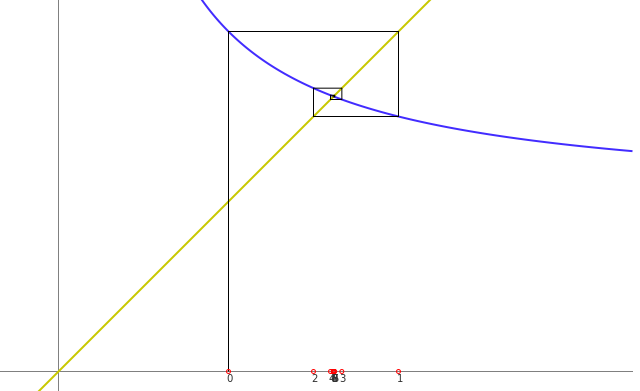
\includegraphics[width=\textwidth]{fig_fibonacci.png}
  \end{center}
  \caption{Spider diagram related
    to exercise~\ref{ex_fibonacci}:
    on the ratio of successive terms of the Fibonacci sequence.\\\\
    \usebox{\qrexfibonacci}%
    }
  \label{fig_fibonacci}
\end{figure}

A graphical method to visualize the behavior of the
sequence defined by \eqref{eq1} is the \emph{spider diagram}. One draws the
curve $y=f(x)$ on a Cartesian plane.
Starting from the point with coordinates $(\alpha, 0)=(a_0, 0)$, one proceeds
along a vertical line until reaching the graph of the function
at the point $(a_0, f(a_0)) = (a_0, a_1)$.
Then, one proceeds horizontally until intersecting the line $y=x$ at the point
$(a_1,a_1)$ and
repeats the process so that the $x$-coordinates (but also the $y$-coordinates)
of the vertices of the broken line give the sequence $a_0, a_1, a_2,
\dots$. For example, the spider diagram corresponding
to exercise~\ref{ex_fibonacci} is shown in
Figure~\ref{fig_fibonacci}.

\begin{exercise}\label{ex_3}
  Consider the sequence defined recursively by
  \[
  \begin{cases}
    a_0 = 0\\
    a_{n+1} = 1 + a_n^2.
  \end{cases}
  \]
  Determine the limit of the sequence.
\end{exercise}
\newsavebox{\qrextre}\sbox{\qrextre}{%
\myqrshortdoclink{ex3}{Spider diagram related to exercise \getrefnumber{ex_3}}}
\begin{figure}
  \begin{center}
    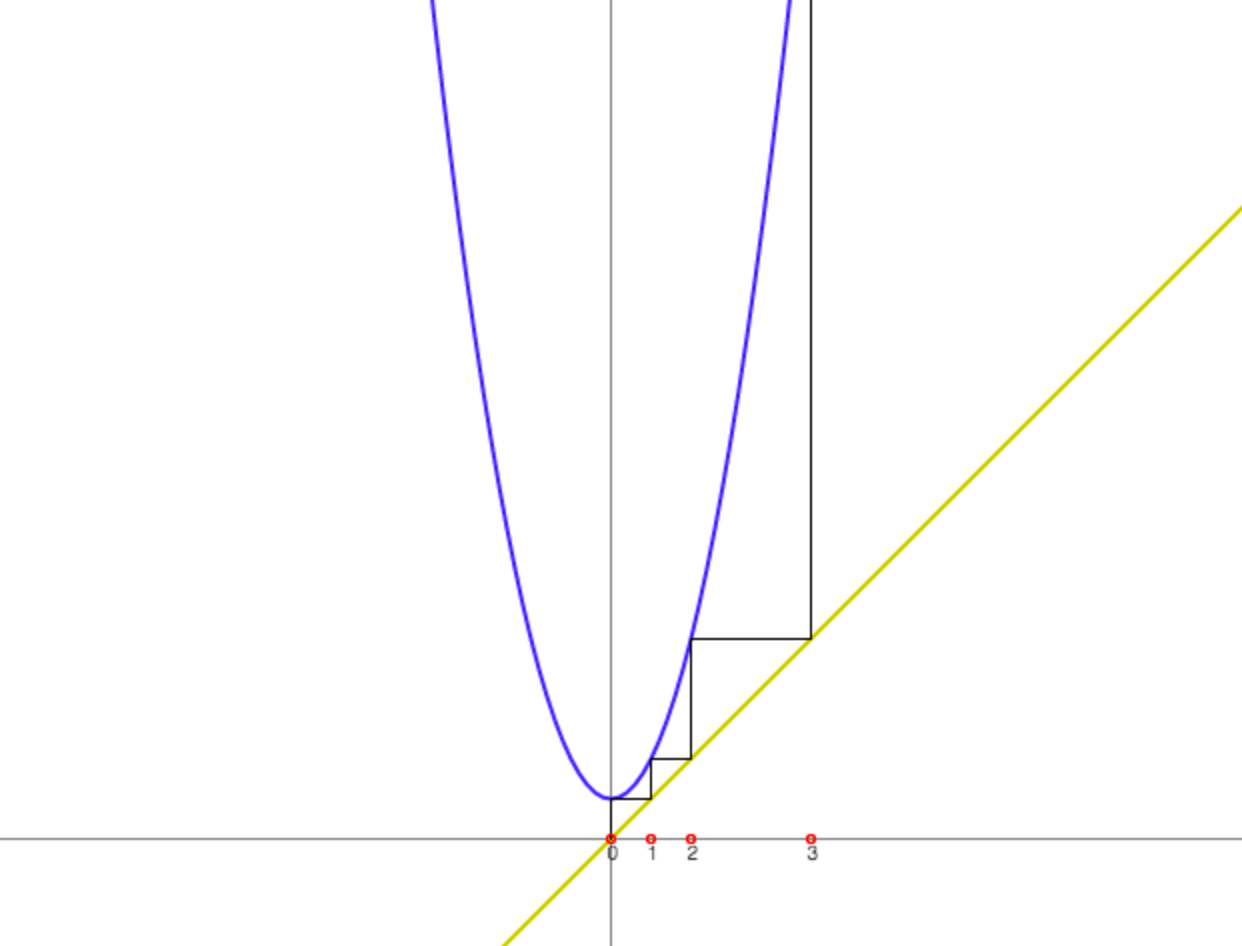
\includegraphics[width=\textwidth]{fig_ex_3.png}
  \end{center}
  \caption{Spider diagram related
    to exercise~\ref{ex_3}.
    \ifwidemargin\\\\\fi%
    \usebox{\qrextre}}
  \label{fig_ex_3}
\end{figure}

\begin{proof}[Solution]
  The recursive equation is $a_{n+1}=f(a_n)$ if we set $f(x) = 1+x^2$.
  It is easy to verify that for every $x$, we have $f(x) > x$, and thus, by
  Theorem~\ref{th_1}, we obtain that the sequence $a_n$ is
  increasing. Therefore, it admits a limit: $a_n \to \ell$. If the limit were
  finite, we would have
  \[
  a_{n+1} = 1 + a_n^2 \to 1 + \ell^2
  \]
  and thus, since $a_{n+1}\to \ell$, we would have $\ell = 1 +
  \ell^2$ (i.e., $\ell$ should be a fixed point of $f$). This
  equation we have already observed has no solutions ($x^2 + 1 > x$),
  and thus $\ell$ is not finite. Since the sequence $a_n$ is
  increasing, we can exclude that $\ell=-\infty$, and thus the only
  possibility remaining is that $a_n \to +\infty$.
\end{proof}

\newsavebox{\qrexquattro}\sbox{\qrexquattro}{%
\myqrshortdoclink{ex4}{Spider diagram related to exercise \getrefnumber{ex_4}}}
\begin{figure}
  \begin{center}
  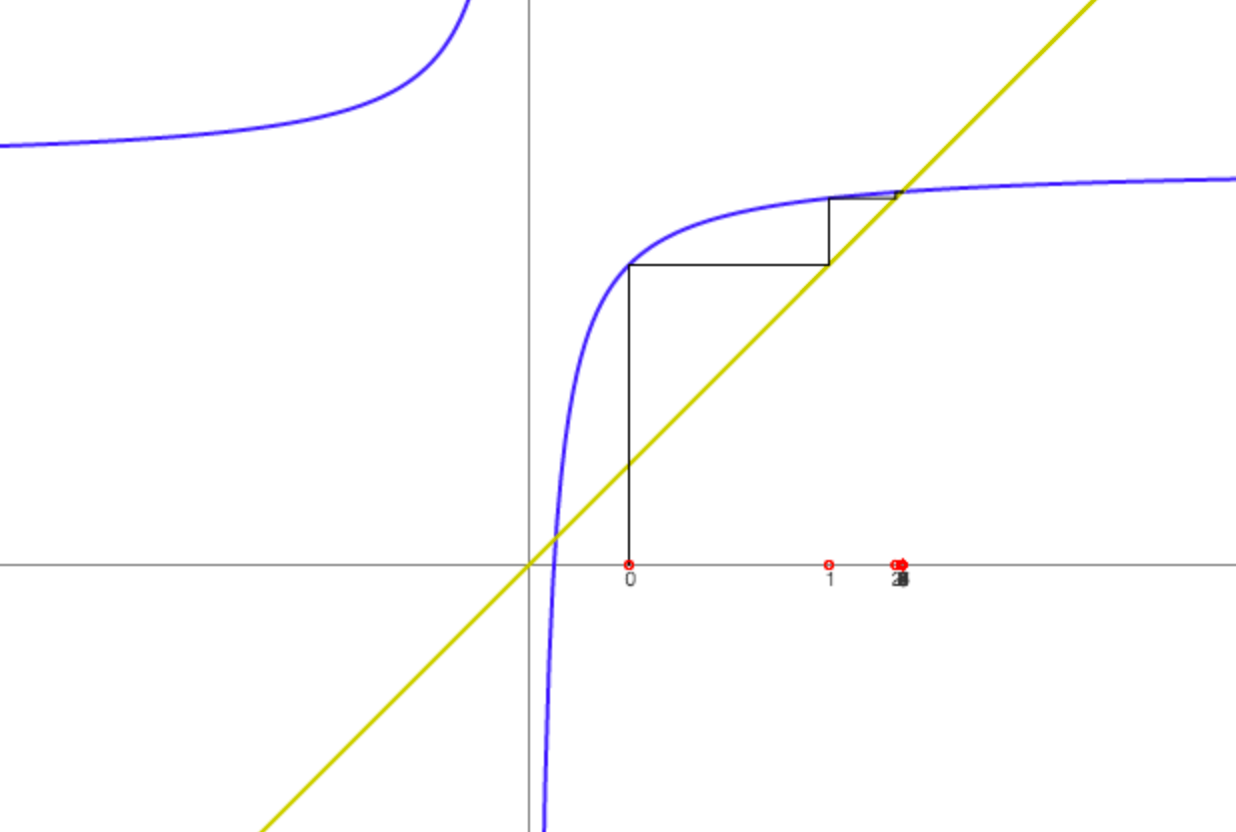
\includegraphics[width=\textwidth]{fig_ex_4.png}
  \end{center}
  \caption{Spider diagram related
    to exercise~\ref{ex_4}.
    \ifwidemargin\\\\\fi%
    \usebox{\qrexquattro}
    }
  \label{fig_ex_4}
\end{figure}

\begin{exercise}\label{ex_4}
  Consider the sequence defined recursively by
  \[
  \begin{cases}
    a_0 = 1\\
    a_{n+1} =4-\frac 1 {a_n}.
  \end{cases}
  \]
  Determine the limit of the sequence.
\end{exercise}

\begin{proof}[Solution]
  It is shown that on the interval $A=(2-\sqrt 3, 2+\sqrt 3)$,
  it holds that $f(x)>x$, that the endpoints of $A$ are fixed points,
    and moreover, that the function $f$ is increasing (it is on the entire
  $(0,+\infty)$).
  Consequently, it is easy to verify that $A$ is invariant since
  \begin{align*}
  2-\sqrt 3 < x < 2+\sqrt 3 &\Rightarrow
  f(2-\sqrt 3) < f(x) < f(2+\sqrt 3)\\
  &\Rightarrow
  2-\sqrt 3 < f(x) < 2+\sqrt 3.
  \end{align*}

    Moreover, if $a_0 \in A$, then for every $n\in\NN$, we have $a_n\in A$, and
  since
  $f(x)>x$, the sequence will be increasing. Thus, it admits
  a limit: $a_n \to \ell \in [2-\sqrt 3,2+\sqrt 3]$, $\ell \ge a_0$.
  But then
  \[
  a_{n+1} = 4-\frac 1 {a_n} \to 4 - \frac 1 \ell = f(\ell)
  \]
  and since $a_{n+1}$ has the same limit as $a_n$, we have $\ell =
  f(\ell)$, whose only solutions are $2\pm \sqrt 3$. But $2-\sqrt 3$
  must be discarded since $\ell\ge a_0 > 2-\sqrt 3$, and thus remains
  $a_n \to \ell = 2+\sqrt 3$.
\end{proof}

\newsavebox{\qrexcinque}\sbox{\qrexcinque}{%
\myqrshortdoclink{ex5}{Spider diagram related to exercise \getrefnumber{ex_5}}}
\begin{figure}
 \begin{center}
    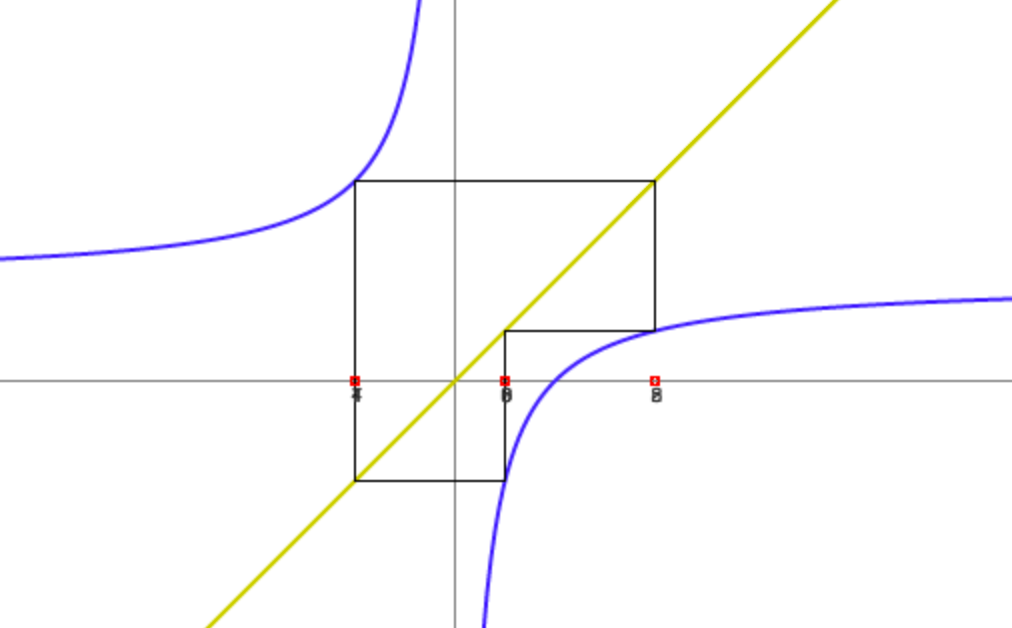
\includegraphics[width=\textwidth]{fig_ex_5.png}
  \end{center}
  \caption{Spider diagram related
    to exercise~\ref{ex_5}.
    \ifwidemargin\\\\\fi%
    \usebox{\qrexcinque}}
  \label{fig_ex_5}
\end{figure}

\begin{exercise}\label{ex_5}
  Consider the sequence defined recursively by
  \[
  \begin{cases}
    a_0 = \frac 1 2\\
    a_{n+1} = 1 - \frac{1}{a_n}
  \end{cases}
  \]
  Determine, if it exists, the limit of the sequence.
\end{exercise}

\begin{proof}[Solution]
  Observe that:
  \begin{align*}
    a_0 &= \frac 1 2 \\
    a_1 &= 1 - \frac{1}{1/2} = -1\\
    a_2 &= 1 - \frac{1}{-1} = 2\\
    a_3 &= 1 - \frac{1}{2} = \frac 1 2 = a_0
  \end{align*}
  Since $a_3 = a_0$, the sequence repeats, and (by induction), it
  is shown that $a_{3n+k} = a_k$. Thus, we have
  \begin{align*}
    a_{3n} &= a_0 = \frac 1 2\\
    a_{3n+1} &= a_1 = -1\\
    a_{3n+2} &= a_2 = 2
  \end{align*}
  and the sequence $a_n$ does not admit a limit.
\end{proof}

\newsavebox{\qrexsei}\sbox{\qrexsei}{%
\myqrshortdoclink{ex6}{Spider diagram related to exercise \getrefnumber{ex_6}}}
\begin{figure}
  \begin{center}
    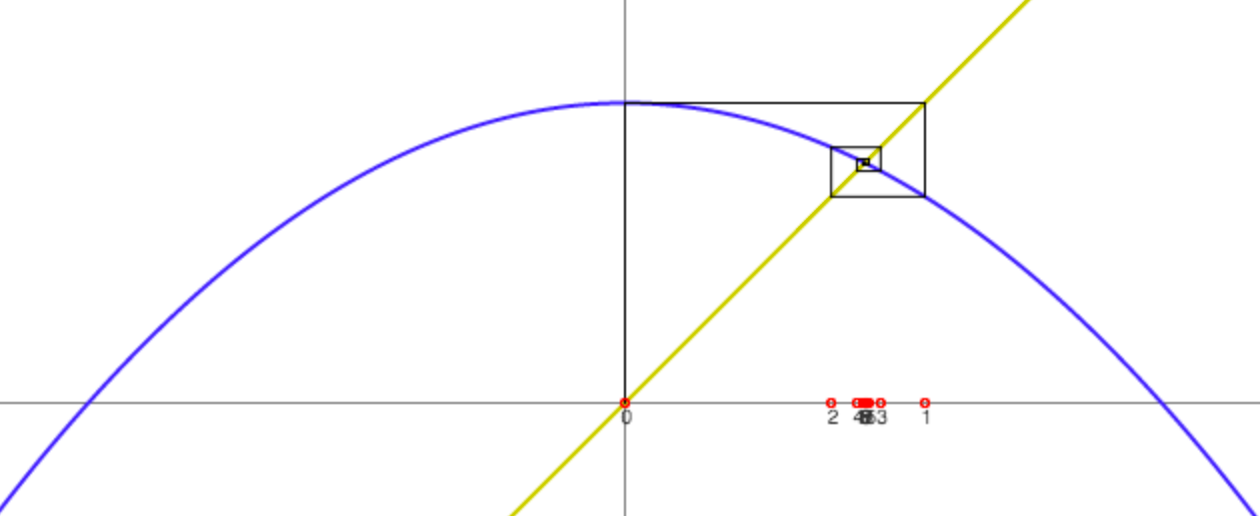
\includegraphics[width=\textwidth]{fig_ex_6.png}
  \end{center}
  \caption{Spider diagram related
    to exercise~\ref{ex_6}.
    \ifwidemargin\\\\\fi%
    \usebox{\qrexsei}}
  \label{fig_ex_6}
\end{figure}

\begin{exercise}\label{ex_6}
  Consider the sequence defined recursively by
  \[
  \begin{cases}
    a_0 = 0\\
    a_{n+1} = \frac{5-a_n^2}{4}.
  \end{cases}
  \]
  Determine the limit of the sequence.
\end{exercise}

\begin{proof}[Solution]
We have $a_{n+1} = f(a_n)$ if we choose $f(x) = (5-x^2)/4$. Observe
that the function $f$ is decreasing for $x \ge 0$ (indeed, $0 \le x_1 <
x_2$ implies $x_1^2 < x_2^2$, from which $-x_1^2 > -x_2^2$, and thus $f(x_1)
> f(x_2)$). Also observe that
\begin{align*}
a_0 &= 0\\
a_1 &= f(a_1) = \frac 5 4.\\
a_2 &= f\enclose{\frac 5 4} = \frac{5-25/16}{4} = \frac{55}{64}
\end{align*}
We want to show that the interval $A=[0,5/4]$ is invariant. Since
$f$ is decreasing on this interval, we have:
\begin{align*}
0 \le x \le \frac 5 4 &\Rightarrow f(0) \ge f(x) \ge f(5/4)\\
&\Rightarrow \frac 5 4 \ge f(x) \ge \frac{55}{64} \ge 0\\
&\Rightarrow 0 \le f(x) \le \frac 5 4
\end{align*}
i.e., $x\in A \Rightarrow f(x)\in A$, which is what we wanted to show.

By Theorem~\ref{th_decr}, we know that $a_{2n} \to \ell$ and
$a_{2n+1} \to \ell'$. Both limits are finite since $a_n \in A$ for every $n$, so
$\ell, \ell' \in \bar A = A$.
Thus, as usual, we observe that:
\begin{align*}
  a_{2n+1} &= f(a_n) \to f(\ell)  \\
  a_{2n+2} &= f(a_{n+1}) \to f(\ell')
\end{align*}
but knowing that $a_{2n+1}\to \ell'$ and $a_{2n+2}\to \ell$, we obtain the
following system:
\[
\begin{cases}
  \ell' = f(\ell)\\
  \ell = f(\ell')
\end{cases}
\]
from which we obtain $f(f(\ell))=\ell$ and $f(f(\ell'))=\ell'$. Thus
we want to write and solve the equation $f(f(x))=x$:
\[
\frac{5-\left(\frac{5-x^2}{4}\right)^2}{4} = x
\]
i.e.,
\[
5 - \frac{25 - 10x^2 + x^4}{16} = 4x
\]
or
\[
x^4 - 10 x^2 + 64 x - 55 = 0.
\]

How do we solve a quartic equation?
In this context, we need to make a general observation that will be of great
help.
Observe that if $x$ is a solution of $f(x)=x$, then $x$
is also a solution of $f(f(x)) = x$ since in that case, we have
$f(f(x))=f(x)=x$.
But the equation $f(x) = x$ is a quadratic equation, which we can easily solve:
\begin{gather*}
  \frac{5-x^2}{4} = x \\
  x^2 + 4x - 5 = 0 \\
  x_{12} = -2 \pm \sqrt{4 + 5} = -2 \pm 3.
\end{gather*}

Thus, we have found two zeros of the quartic polynomial, and
such a polynomial must therefore be divisible by
\[
 x^2 + 4x - 5 = (x-1)(x+5).
\]
We perform the polynomial division:
\begin{align*}
\frac{x^4 - 10 x^2 + 64 x - 55}{x^2 + 4x - 5}
&= x^2 + \frac{x^4 - 10 x^2 + 64x - 55 - x^2 (x^2 + 4x - 5)}{x^2+4x-5}\\
&= x^2 + \frac{-4x^3 - 5 x^2 + 64 x - 55}{x^2+4x-5}\\
&= x^2 - 4x + \frac{-4x^3 - 5x^2 - 64 x - 55 + 4x(x^2+4x-5)}{x^2+4x-5}
\\
&= x^2 - 4x + \frac{11 x^2 + 44 x - 55}{x^2 + 4x -5}\\
&= x^2 - 4x + 11.
\end{align*}
As expected, the division has no remainder. We can therefore complete the
factorization by finding the zeros of the polynomial $x^2-4x+11$, which, upon
quick inspection, has no real solutions.

Thus, in this case, the fixed points of $f$ coincide with the fixed
points of $f\circ f$, and thus the two limits $\ell, \ell'$ must be
elements of the set of fixed points: $\ENCLOSE{1, -5}$. On the other hand, $-5$
must be excluded since the limits both lie in the closure of the
invariant set, which does not include negative numbers.

We conclude, therefore, that $\ell = \ell' = 1$, and thus the entire
sequence has a limit: $a_n \to 1$.
\end{proof}

\begin{exercise}\label{ex_7}
  %% a_n <- (a_n + 2)/4
  Consider the sequence defined recursively by
  \[
  \begin{cases}
    a_0 = \alpha\\
    a_{n+1} = 4 a_n (1-a_n) % 2- a_n^2.
  \end{cases}
  \]
  Determine the limit of the sequence in the cases: 
  $\alpha=-1$, 
  $\alpha=2$, and 
  $\alpha=1/42$.
\end{exercise}


\newsavebox{\qrexsette}\sbox{\qrexsette}{%
\myqrshortdoclink{ex7b}{Spider diagram related to exercise \getrefnumber{ex_7}}}
\begin{figure}
   \begin{center}
    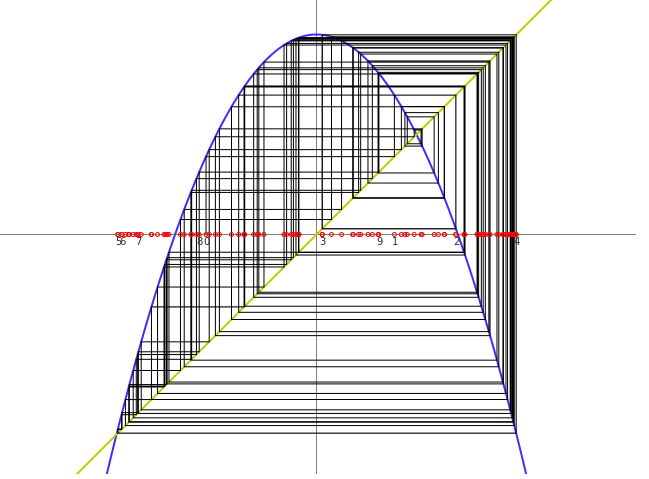
\includegraphics[width=0.5\textwidth]{fig_ex_7.png}
  \end{center}
  \caption{Spider diagram related
    to exercise~\ref{ex_7}.
    \ifwidemargin\\\\\fi%
    \usebox{\qrexsette}}
  \label{fig_ex_7}
\end{figure}

\begin{proof}[Solution]
  We have $a_{n+1} = f(a_n)$ with $f(x) = 4x(1-x)$. 
  We determine the fixed
  points of $f$:
  \[
  4x(1-x)= x, \qquad 4 x^2 - 3x = 0
  \]
  which has solutions $x_1=0$ and $x_2=\frac 3 4$. 
  Taking into account the signs, it can be
  observed that within the two solutions, $f(x)>x$, while
  outside, $f(x)<x$.

  Also observe that $f(x)$ is increasing for
  $x\le \frac 1 2$ and decreasing for $x\ge \frac 1 2$.

  Case $\alpha=-1$. In this case, consider the interval
  $A=(-\infty, 0)$. Since $f$ is increasing on this interval,
  and since $0$ is a fixed point, we have:
  \[
  x < 0 \Rightarrow f(x) < f(0) \Rightarrow f(x) < 0
  \]
  which means that $A$ is an invariant interval.

  On this interval, $f(x)<x$, and thus $a_n$ is decreasing, and
  consequently, it admits a limit $a_n\to \ell$. The limit can be
  finite or $-\infty$. But if it were finite, then we would have
  \[
  a_{n+1} = 4 a_n (1-a_n) \to 4 \ell (1-\ell)
  \]
  and since $a_{n+1}\to \ell$, we would have that $\ell$
  is a fixed point of $f$. 
  But since $\ell \le a_0 = \alpha < 0$,
  we obtain a contradiction.

  Thus, the only possibility is that $a_n \to -\infty$. This
  same reasoning applies for any $\alpha<0$.

  Case $\alpha=2$. In this case, we have:
  \begin{align*}
    a_0 &= \alpha = 2\\
    a_1 &= f(a_0) = 4\cdot 2\cdot (1-2) = -8.
  \end{align*}
  so $a_1 \in A$ (the invariant interval from the previous point), and
    from index $2$ onward, we thus reduce to the previous results. Thus, in this
  case as well, $a_n \to -\infty$.

  Case $\alpha = \frac 1{42}$. This case is decidedly more complex than
    the previous ones. Consider the set $A_2 = [0, 1]$: we want to show that it
  is an invariant set. In the interval $\closeinterval{0}{\frac 1 2}$, the
  function is
    increasing, and thus it has a minimum at $0$, where it takes the value
  $f(0)=0$, and it has
    a maximum at $\frac 1 2$, where it takes the value $f(1/2) = 1$. In the
  interval
    $\closeinterval{\frac 1 2}{1}$, the function is decreasing, and again, it
  has a maximum $f(1/2)=1$ and
  a minimum $f(1)=0$. Thus, for every $x\in [0,1]$, we have $f(x) \in
  [0,1]$, i.e., as we wanted to show, $A_2$ is invariant.

  Thus, since $a_0 = \alpha \in A_2$, we find that for every $n$,
  $a_n \in [0,1]$. Suppose now that the sequence has
  a limit: $a_n \to \ell$. In this case, taking the limit
  in the equation $a_{n+1} = f(a_n)$, we obtain, as usual, that the
  limit should be a fixed point of $f$: either $\ell=0$ or
    $\ell=\frac 3 4$. We will now try to show that this is absurd. There are two
  possibilities that we need to exclude. The first is that the
  sequence tends to the fixed point $\ell$ without ever equaling it. The
  second is that for a certain $n_0$, we have $a_n = \ell$ for $n=n_0$ and
  thus for every $n\ge n_0$.

  Suppose we are in the first case and suppose that $\ell = 0$. In
    this case, by the permanence of sign theorem, the sequence must, from a
  certain index onward, stay in the interval $\closeinterval{0}{\frac 1 2}$. But
  in this interval, $f(x)>x$, and thus the sequence would be,
  from a certain index onward, increasing. But since $a_n \ge 0$ for
  every $n$, it is not possible for the sequence to converge, increasing, to
  $0$.

  Suppose then we are in the first case (the sequence is always
  different from the two fixed points) and suppose that $\ell = \frac 3 4$. In
  this case, from a certain index onward, the sequence must stay
    in the interval $\closeinterval{\frac 1 2}{1}$ (otherwise, it could not
  converge to
  $\frac 3 4$). In this interval, the function $f$ is decreasing, and thus
  the subsequences of even-indexed and odd-indexed terms are
  both monotone. One could try to study the sequences of
    even-indexed terms $a_{2n}$ and odd-indexed terms $a_{2n+1}$ that satisfy a
  recurrence relation
  with the function $f\circ f$ instead of $f$ and observe that the sequence
    on the left of the fixed point should decrease, and the one on the right
  should increase (and this would be absurd). A perhaps more
    rapid method that does not require the study of the composed function is
  instead the following.
    The idea is to observe that $f$ tends to increase the distances when one is
  near
    the point $1$. If, for the sake of contradiction, $a_n\to \frac 3 4$, then
  definitely
  it must be $\abs{a_n-\frac 3 4}< 1/8$. But then it is observed that:
  \[
    \abs{a_{n+1}-\frac 3 4}
    = \abs{4a_n(1-a_n)-\frac 3 4}
    = \abs{\frac 3 4 - 4a_n + 4a_n^2}
    = \abs{a_n-\frac 3 4}\abs{4a_n -1}
    \ge 4\abs{a_n-\frac 3 4}
  \]
  since if $\abs{a_n-\frac 3 4}<1/8$, then (by the reverse triangle inequality)
    $\abs{4a_n-1}\ge 4$. This is absurd because it means that $\abs{a_n -\frac 3
  4}\to +\infty$
  (by the ratio test) when instead it should be $\abs{a_n-\frac 3 4}\to 0$.

  \textbf{Note.} We will see in the upcoming theorems that
  if the derivative of $f$ is in absolute value less than
  $1$, then the fixed point will be stable (or attractive), i.e., starting
  from a point sufficiently close, one will necessarily converge to
  the fixed point. If instead the derivative is in absolute value greater than
  $1$, the fixed point will be unstable (or repulsive). That is, apart from the
  constant sequence that takes the exact value of the fixed point,
  it is
  not possible for a sequence to converge to the fixed point.

  It remains to consider the possibility that the sequence takes from a
  certain point onward the exact value of a fixed point. Suppose, for
  example, that for a certain $n$, we have $a_n=\frac 3 4$. Then it must be
  \[
  \frac 3 4 = a_n = 4\cdot a_{n-1} \cdot (1-a_{n-1})
  \]
  from which we derive (via~\eqref{eq:secondo_grado})
  \[
  a_{n-1} = \frac 3 4 
  \qquad\lor\qquad
  a_{n-1} = \frac 1 4.
  \]
  If $a_n$ was the first term with value $\frac 3 4$, it must necessarily
  be $a_{n-1} = \frac 1 4$. But then
  \[
  \frac 1 4 = a_{n-1} = 4 a_{n-2}(1-a_{n-2})
  \]
  from which $a_{n-2} = \frac{2\pm\sqrt 3}{4}$. But now observe that since $a_0=
  \alpha = \frac 1 {42}$ is a rational number, and observing that $\QQ$ is an
  invariant set for $f$ (why? verify by induction...)
  we deduce that every $a_k \in \QQ$, and thus
  we would have $a_{n-2} = \frac{2\pm\sqrt 3}{4} \in \QQ$: absurd.

  The same reasoning applies if we had $a_n=0$, since we
    would have $a_{n-1} = 1$, $a_{n-2} = \frac 1 2$, and thus $a_{n-3}=\frac{2
  \pm \sqrt 2}{4}$.

  Thus, the sequence $a_n$ does not admit a limit.
\end{proof}

\begin{exercise}\label{ex_8}
  Consider the sequence defined recursively by
  \[
  \begin{cases}
    a_0 = \alpha\\
    a_{n+1} = \frac{1}{2-a_n}.
  \end{cases}
  \]
  Find the limit of the sequence in the case $\alpha =
  -\the\year$. Determine the set of values of $\alpha$ for which the
  sequence $a_n$ is not well-defined (since for some $n$, the
  denominator $2-a_n$ becomes zero).
  Find the limit in the case $\alpha=\frac{\the\year}{1000}$.
\end{exercise}

\newsavebox{\qrexotto}\sbox{\qrexotto}{%
\myqrshortdoclink{ex8}{Spider diagram related to exercise \getrefnumber{ex_8}}}
\begin{figure}
 \begin{center}
    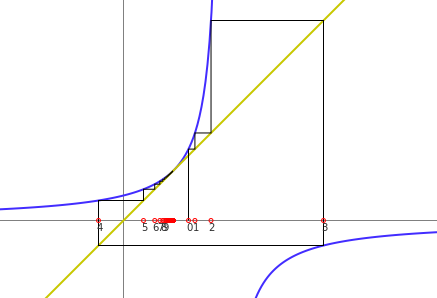
\includegraphics[width=\textwidth]{fig_ex_8.png}
  \end{center}
  \caption{Spider diagram related
    to exercise~\ref{ex_8}.
    \ifwidemargin\\\\\fi%
    \usebox{\qrexotto}}
  \label{fig_ex_8}
\end{figure}

\begin{proof}[Solution]
Setting $f(x) = 1/(2-x)$,
it is observed that the inequality $f(x)\ge x$ is satisfied for every
$x<2$. The fixed point equation $f(x)=x$ has as its only solution
$x=1$. On the interval $A=(-\infty,1)$, the function $f$ is increasing, and
the interval is invariant. Thus, for
$\alpha=-\the\year \in A$, the sequence is increasing and bounded above. Thus,
it converges $a_n\to \ell$. Taking the limit in
$a_{n+1} = f(a_n)$, we find that $\ell$ must be a fixed point of
$f$, and thus $\ell = 1$.

The sequence is not well-defined if for some $n$, we find
$a_n=2$, since the function $f$ is not defined for $x=2$. Other
values are obtained by tracing the sequence $a_n$ backward.
From the equation
\[
a_n = \frac{1}{2-a_{n-1}}
\]
we derive
\[
a_{n-1} = 2-\frac{1}{a_n}.
\]
The set of points from which one eventually reaches $x=2$ is
given by the values of the sequence
\[
\begin{cases}
  b_1 = 2\\
  b_{n+1} = 2 - \frac{1}{b_n}.
\end{cases}
\]
Observe that in this specific case, it is possible to derive an
explicit formula for the term $b_n$. Indeed, observe that:
\[
b_0 = 2,\quad
b_1 = \frac{3}{2},\quad
b_2 = \frac{4}{3}
\]
and we conjecture that $b_n = \frac{n+1} n$. Indeed, this
can be proven by induction. For $n=1$, we have $(n+1)/n = 2 =
b_1$. And if we assume that $b_n = (n+1)/n$, we have
\[
b_{n+1} = 2 - \frac{n}{n+1} = \frac{2n+2-n}{n+1} = \frac{n+2}{n+1}.
\]
Thus, the set of points from which the sequence $a_n$ is not
well-defined is given by:
\[
  X= \ENCLOSE{\frac{n+1}{n}\colon n \in \NN}.
\]

For the case $\alpha=\frac{\the\year}{1000}$, observe that on the interval
$A_2 = (1,2)$, it always holds that $f(x)>x$ (but it could be observed that
$A_2$ is not invariant). As long as $a_n$ remains in
this interval, the sequence is thus increasing. However, it is
not possible for the sequence to always remain in $A_2$ because in such
a case, the limit should be a fixed
point. But the only fixed point is $1$, which is less than $\alpha$, and thus
the sequence, being increasing, cannot converge. Necessarily, the
sequence exits the interval $A_2$ (indeed, note that $\alpha
\not \in X$), and for a certain $n$, we will have $a_n>2$. Observe now that
on the interval $A_3 = (2,+\infty)$, it holds that $f(x)<0$, and thus
if $a_n\in A_2$, necessarily $a_{n+1} \in A$. Thus, this case is
reduced to the first studied, and the sequence tends to $1$.
\end{proof}

\begin{exercise}
  Consider the sequence defined recursively by
  \[
  \begin{cases}
    a_0 = \alpha\\
    a_{n+1} = \frac{a_n^2-a_n}{2}.
  \end{cases}
  \]
  Determine, as $\alpha$ varies, the limit of the sequence.
\end{exercise}

\begin{exercise}
  Consider the sequence defined recursively by
  \[
  \begin{cases}
    a_0 = \alpha \\
    a_{n+1} = 1 - a_n^2.
  \end{cases}
  \]
  Determine, as $\alpha$ varies, the limit of the sequence.
\end{exercise}

\begin{exercise}
  Calculate the limit of the sequence $a_n$ 
  defined recursively by:
    \[
    \begin{cases}
      a_0 = 1\\
      a_{n+1} = 1 - \frac {4}{a_n^2}.
    \end{cases}
    \]
  \end{exercise}
  
\begin{exercise}
  Calculate the limit of the sequence $a_n$
  defined recursively by:
  \[
    \begin{cases}
      a_0 = 10\\
      a_{n+1} = a_n \cdot (\abs{a_n}-1).
    \end{cases}
  \]
\end{exercise}
  
\begin{exercise}
Calculate
\[
 1 + \frac{1}{1+\frac{1}{1+\frac{1}{1+\frac{1}{\dots}}}}
\]
\end{exercise}

\begin{exercise}
Calculate
\[
  \lim_{x\to 1^+} \sqrt{x-\sqrt{x- \sqrt{x-\sqrt{x - \dots}}}}
\]
\end{exercise}

\begin{exercise}[Real Mandelbrot]
\label{ex:mandelbrot_reale}
Consider, with the parameter $c$ fixed, the sequence defined recursively:
\[
  \begin{cases}
    a_0 = 0\\
    a_{n+1} = a_n^2 + c.
  \end{cases}
\]

Determine the values of $c\in \RR$ for which the sequence $a_n$ is
bounded.
\end{exercise}
%
\begin{proof}[Solution.]
\emph{Case 1: $c > \frac 1 4$}.
In this case, there are no fixed points, as the equation $x=x^2+c$ has
a negative discriminant. This means that $x^2+c > x$ for every $x\in \RR$. Thus,
the sequence $a_n$ is strictly increasing and tends to $+\infty$.
It is not bounded.

\emph{Case 2:} $0\le c \le \frac 1 4$.
In this case, the equation $x=x^2+c$ has two solutions, both positive
(the solutions have sum $1$ and product $c\ge 0$).
If we call $x_1$ the smaller of the two solutions, we can show that
the interval $[0,x_1)$ is invariant. Indeed, on such an interval, the function
$f(x)=x^2+c$ is increasing, so if $0\le x < x_1$, we have $f(0) \le f(x) <
f(x_1)$,
i.e., $c \le f(x) < x_1$. Since $c\ge 0$, we have shown that the interval is
invariant, and the sequence is thus bounded.
If $c=0$, the sequence $a_n$ remains constant $a_n=0$. If $c>0$, the sequence
converges to the fixed point $x_1$. In any case, it is bounded.

\emph{Case 3:} $-1 \le c < 0$.
In this case, we want to show that the interval $[c,0]$ is invariant.
The function $f(x) = x^2+c$ is decreasing on this interval, so
if $c\le x \le 0$, we have $f(0)\le x \le f(c)$. But $f(0)=c$ and $f(c)=c^2+c
= c(c+1) \le 0$ if $c\ge -1$. Thus, $[c,0]$ is invariant, and $a_n$ remains
bounded in this interval.

\emph{Case 4:} $-2\le c < -1$.
In this case, the equation $x=x^2+c$ has one negative solution and one positive
solution.
Call $x_2$ the positive solution. We want to show that
the interval $[c,x_2]$ is invariant.
The function $f(x)=x^2+c$ is decreasing in $[c,0]$ and increasing in $[0,x_2]$.
If $0\le x \le x_2$, we have $f(0)\le f(x) \le f(x_2)$,
i.e., $c \le f(x) \le x_2$. Thus, points in $[0,x_2]$ remain in the interval
$[c,x_2]$.
If instead $c\le x \le 0$, we have $f(0)\le f(x) \le f(c)$, i.e., $c \le f(x)
\le c^2+c$.
To ensure $c^2+c\le x_2$, it suffices to verify that $f(c^2+c)\le c^2+c$,
i.e.,
\[
  (c^2+c)^2 + c \le c^2+c
\]
which, expanding the square, reduces to $c^3(c+2)\le 0$, which is satisfied
if $-2 \le c \le 0$.
Thus, the interval $[c,x_2]$ is invariant. The sequence remains thus
bounded in this interval.

\emph{Case 5:} $c < -2$.
In this case, $a_0=0$, $a_1=c$, $a_2=c^2+c$, and we can verify that
$c^2+c > x_2$ since, as in the previous case, this occurs if
\[
   (c^2+c)^2 + c > c^2+c
\]
which reduces to $c^3(c+2)>0$, which is satisfied if $c<-2$.
But the interval $(x_2,+\infty)$ is invariant, and on this interval,
we have $f(x)>x$, so the sequence $a_n$ is strictly increasing for $n\ge 2$
and diverges to $+\infty$. It is thus not bounded.

\emph{Conclusion}. The sequence is bounded if $c\in[-2,1/4]$.
Otherwise, $a_n\to +\infty$.

\end{proof}